Given a holomorphic function $f(z)$ defined on an annulus $0 \leq R_2 < \abs{z} < R_1 \leq \infty$, we can always find its Laurent series. This means that there exists coefficients $a_n$ for $n \in \Z$ so that 
$$f(z) = \sum_{n = -\infty}^\infty a_n z^n$$
for $z$ in the annulus. Such a series converges if series with negative indices and non-negative indices converge separately. 

Let $\gamma_1$ and $\gamma_2$ be the boundary of a disk of radius $r_1$ and $r_2$ respectively where $R_2 < r_2 < r_1 < R_1$. By Cauchy's Integral formula we get
$$f(z) = \frac{1}{2\pi i} \int_{\gamma_1} \frac{f(\zeta)}{\zeta - z} d\zeta - \frac{1}{2\pi i} \int_{\gamma_2} \frac{f(\zeta)}{\zeta - z} d\zeta$$
We have already seen above how to express the first integral as a series. For the second integral we can write $(\zeta - z)^{-1} = - z^{-1}(1 - \frac{\zeta}{z})^{-1}$ and expand this using the geometric series. In this case we get that the $a_n$ are the exact same except we are integrating over $\gamma_2$ instead. In summary, we can write
$$f(z) = \sum_{n = -\infty}^{\infty} a_n z^n$$
where 
$$a_n = \frac{1}{2\pi i} \int_{\gamma_i} \frac{f(\zeta)}{\zeta^{n + 1}} d\zeta$$
where $i = 1$ if $n \geq 0$ and $i = 2$ if $n < 0$.
This series converges uniformly and absolutely in $r_2 \leq \abs{z} \leq r_1$. The portion of the Laurent series with the negative indices is called its principal part. We can use the Laurent series to prove some very nice statements.

\begin{theorem}
A meromorphic function $f(z)$ on $S^2$ is rational.
\end{theorem}
\begin{proof}
    Since $S^2$ is compact, there can only be finitely many poles say $b_1, \dots, b_k$ and possibly $\infty$. The corresponding principal parts are $P_j(\frac{1}{z - b_j})$ for each of the $b_j$ and $P_\infty(\frac{1}{\zeta})$ where $\zeta$ is the coordinate at $\infty$. Since $\zeta = 1/z$, $P_\infty$ is actually a polynomial in $z$. Then we see that
    $$f(z) - P_\infty(z) - \sum_{j = 1}^k P_j \left( \frac{1}{z - b_j} \right)$$
    is a holomorphic function on $S^2$. Moreover since $S^2$ is compact it must also be bounded. But then Liouville's Theorem allows us to conclude that $f$ is actually constant. Therefore
    $$f(z) = c + P_{\infty}(z) + \sum_{j = 1}^k P_j \left( \frac{1}{z - b_j} \right)$$
    is rational. In fact, this even gives us the partial fraction decomposition of the rational function.
\end{proof}

If we a holomorphic function defined on a punctured neighbourhood of 0 (i.e. on $0 < \abs{z} < R$) then 0 is said to be an isolated singularity. If $f$ extends holomorphically to 0, then 0 is said to be a \textit{removable} singularity. We have such an extension if and only if $f$ is bounded in a (punctured) neighbourhood of 0 (this follows from Cauchy's inequalities which still hold for coefficients in the Laurent expansion and allows us to show that all the negative index coefficients must be 0). 

If $f$ does not extend holomorphically to 0 then there are essentially 2 different behaviours of $f$ (at 0), which are determined by the Laurent series. If the Laurent series has only finitely many terms with negative indices then we have a \textit{pole} at 0. Otherwise there are an infinite number of terms with negative indices and we have an \textit{essential singularity} at 0.

\begin{theorem}[Weierstrass' Theorem]\label{thm:ess-sing-dense}
    If 0 is an essential singularity, then for any $\epsilon > 0$, we have $f(0 < \abs{z} < \epsilon)$ is dense in $\C$.
\end{theorem}

\subsection{Residue Theorem}
Suppose $f(z)$ is holomorphic. The \textit{residue} of $f(z) dz$ at a point $a$ is defined to be
$$\frac{1}{2\pi i}\int_{\gamma} f(z) dz$$
where $\gamma$ is a curve of winding number 1 (most typically a circle) around $a$. If we write $f(z) = \sum_{n \in \Z} a_n z^n$ then we can immediately compute that the residue of $f(z) dz$ at 0 is $a_{-1}$ (when integrating the other terms disappear since they have a primitive).

The residue at $\infty$ is defined in the exact same way. Let $\gamma$ be a small circle around $z = \infty$. In coordinates at infinity, we can write $\zeta = 1/z$. This means
$$f(z) dz = f(\zeta) \cdot -\frac{1}{\zeta^2} d\zeta$$
If $\gamma$ is a small circle around $\infty$ in the $z$-plane then its image in the $\zeta$-plane is a large circle around 0, with the opposite orientation. Therefore
$$\frac{1}{2\pi i} \int_\gamma f(z) dz = -\frac{1}{2\pi i} \int_{\gamma '} \frac{1}{\zeta^2} f \left( \frac{1}{\zeta} \right) d \zeta$$
Therefore if we have $f(z) = \sum_{n = -\infty}^\infty a_n z^n$ then the residue at $\infty$ is $-a_{-1}$ (in fact one might think the residue would be given by $-a_1$ but the multiplication with $1/\zeta^2$ forces you to shift the index by 2 bringing us back to $-a_{-1}$).

\begin{theorem}[Residue Theorem]
    Let $\Omega$ be an open subset of $S^2$ and $f(z)$ a holomorphic function in $\Omega$ except for isolated singularities which may occur at $\infty$. Let $K$ be a compact subset of $\Omega$ with piecewise $C^1$ boundary $\Gamma$. Then
    $$\int_{\Gamma} f(z) dz = 2\pi i \sum_{z_k \in K} \text{Res}(f, z_k)$$
    where $S$ is the set of singular points of $f$ in $K$. 
\end{theorem}

% TODO: Add Argument Principle

\section{Topology of space of Holomorphic Functions}
Let $\Omega$ be an open neighbourhood of $\C$ (or possibly even $S^2$). Then we use $\mathcal{C}(\Omega)$ to denote the ring of continuous complex-valued functions on $\Omega$ and $\mathcal{H}(\Omega)$ for the subring of holomorphic functions.

There is a natural topology on $\mathcal{C}(\Omega)$ (and therefore on $\Hom(\Omega)$ via the subspace topology). In the study of functions one often defines a topology but defining how a sequence of functions should converge (recall that a metric space is determined completely by its set of convergent sequences). In this case, we will say that a sequence of continuous functions $\{f_n\}$ converges if we have uniform convergence on every compact subset of $\Omega$. More symbolically, we say $\{f_n\}$ converges if, given any compact set $K \subset \Omega$, we have $\{f_n|_K\}$ converges uniformly. 

We can in fact describe the open sets in this topology quite explicitly. Given compact set $K \subset \Omega$ and $\epsilon > 0$, the set 
$$V(K, \epsilon) := \{f \in \Cont(\Omega) : \abs{f(z)}_{z \in K} < \epsilon\}$$ 
is an open neighbourhood of 0. Then the open neighbourhoods of any $g$ can be found by simply translating these. In other words,
$$V(g, K, \epsilon) := \{f \in \Cont(\Omega) : \abs{f(z) - g(z)}_{z \in K} < \epsilon\}$$
is an open neighbourhood of $g$.

If our claim is that this topology is determined by convergent sequences, then we should be able to specify what the metric is. Suppose we cover $\Omega$ by countably many closed disks $D_i$ (for example we can take all the disks of rational radii with centres at rational coordinates). Then we can define
$$\abs{f} = \sum_{i = 1}^\infty \frac{1}{2^i} \min \{ 1, M_i(f) \}$$
where $M_i(f) := \max\{ \abs{f(z)} : z \in D_i \}$. This defines a metric that is translation invariant and in fact induces the above topology. An important remark is that $\Cont(\Omega)$ is complete with respect to this topology.

In order to see this, suppose $\{f_n\}$ form a Cauchy sequence with respect to the above metric. In particular this means that, for any $z \in \Omega$, the sequence $\{f_n(z)\}$ is a Cauchy sequence of complex numbers therefore converges to some value we call $f(z)$. We want to show this pointwise limit is continuous so fix some $z_0 \in \Omega$. There is a compact set $K$ of $\Omega$ containing $z_0$. This compact set is covered by the interiors of finitely many of the $D_i$. This places a bound on $\abs{f(z) - f_n(z)}$ for $z \in K$ [WHAT IS IT] which means that the $f_n$ converge to $f$ uniformly on $K$. Since we know the uniform limit of a sequence of continuous functions is continuous, we know $f$ is continuous at $z_0$.

% TODO: Complete completeness

% TODO: Mention convergence of Taylor series from first-year calc for uniform convergence on compact sets?

\secbreak


Now that we understand the topology on $\Cont(\Omega)$ a bit better, we want to try looking at $\Hom(\Omega)$ as well. In particular, we want to say that $\Hom(\Omega)$ is a closed subset of $\Cont(\Omega)$ and that the differentiation operator is continuous. We translate these into statements about sequences.

\begin{theorem}[Weierstrass]
    If $\{f_n\} \subset \Hom(\Omega)$ is a sequence of holomorphic functions that converges uniformly on compact sets, then $f = \lim_{n \to \infty} f_n$ is holomorphic. Moreover, $\{f_n'\}$ converges uniformly to $f'$ on compact sets.
\end{theorem}
\begin{proof}
    In order to prove the first statement it suffices to show that $f(z) dz$ is closed (see \autoref{thm:holom-tfae}). Let $D$ be an open disk in $\Omega$ and $\gamma$ a closed curve in $D$. Then
    \begin{align*}
        \int_{\gamma} f(z) dz = \lim_{n \to \infty} \int_\gamma f_n(z) dz = 0
    \end{align*}
    where we can swap the limit and integral by uniform convergence. 
    Therefore $f(z) dz$ is closed and by Morera's theorem we know $f(z)$ is holomorphic.

    In order to see that the derivatives converge, let $D$ be a closed disk in $\Omega$. If suffices to show that $f_n'$ converge uniformly to $f'$ on $D$ [TODO: Why?]. Let $\gamma$ be the boundary of a larger circle (than $D$) in $\Omega$. Then for any $z \in D$  we have 
    \begin{align*}
        f'(z) &= \frac{1}{2\pi i} \int_\gamma \frac{f(\zeta)}{(\zeta - z)^2} d\zeta\\
        &= \frac{1}{2\pi i} \int_\gamma \lim_{n \to \infty} \frac{f_n(\zeta)}{(\zeta - z)^2}\\
        &= \lim_{n \to \infty} \frac{1}{2\pi i} \int_\gamma \frac{f_n(\zeta)}{(\zeta - z)^2}\\
        &= \lim_{n \to \infty} f_n'(z)
    \end{align*}
\end{proof}

When speaking of sequences, one must also mention series, i.e. infinite sums. The above statement can also be translated to work with these as well.
\begin{corollary}
If a series of holomorphic functions $\displaystyle \sum_{n = 1}^\infty f_n(z)$ converges uniformly on compact subsets of $\Omega$ to $f(z)$ then $f$ is holomorphic and we can differentiate term by term.
\end{corollary}
\begin{proof}
    Recall a series converges if and only if the partials sum converge. The partial sums are all holomorphic as well therefore if the series converges the limit must be holomorphic, by the above theorem. The second part of the above theorem tells us that the derivatives of the partial sums converge to $f'$ which means exactly that we can compute $f'(z)$ by differentiating the series term by term.
\end{proof}

\begin{proposition}[Hurwitz]\label{lem:hurwitz}
Suppose $\Omega$ is a domain and $\{f_n\} \subset \Hom(\Omega)$ where $f_n$ are all nowhere zero on $\Omega$ and converge uniformly on compact sets. Then either the limit function $f$ is also nowhere zero or it is identically zero on $\Omega$.
\end{proposition}
\begin{remark}
    A domain is an open, connected subset of $\C$. 
\end{remark}
\begin{proof}
    Suppose $f$ is not identically 0. Then since $f$ is holomorphic, its zeroes are isolated. Let $z_0 \in \Omega$ be arbitrary. If it is a zero, we can compute its multiplicity via the Argument Principle
    \begin{align*}
        \int_{\gamma} \frac{f'(z)}{f(z)}dz
    \end{align*}
    where $\gamma$ is a small circle around $z_0$. But then 
    \begin{align*}
        \int_{\gamma} \frac{f'(z)}{f(z)}dz = \int_{\gamma} \lim_{n \to \infty} \frac{f_n'(z)}{f_n(z)}dz = \lim_{n \to \infty} \int_{\gamma} \frac{f_n'(z)}{f_n(z)}dz
    \end{align*}
    where the limit must be 0 since that is multiplicity of $z_0$ as a zero of the $f_n$ for every $n$. Therefore $z_0$ is not a zero of $f$.
\end{proof}

\begin{corollary}\label{cor:hurwitz-cor}
    If $\Omega$ is a domain and $\{f_n\} \subset \Hom(\Omega)$ where $f_n$ are injective and converge uniformly on compact sets to $f$, then $f$ is either constant or also injective.
\end{corollary}
\begin{proof}
    Suppose $f$ is not constant and not 1-1. Then there are distinct points $z_1, z_2 \in \Omega$ so that $f(z_1) = f(z_2) =: a$. Let $V_1, V_2$ be disjoint open neighbourhoods of $z_1$ and $z_2$ respectively. Since $f(z) - a$ vanishes on $V_1$ we know that $f_n$ must have a zero on $V_1$ as well by the previous proposition. But this holds for $V_2$ as well which contradicts injectivity of the $f_n$. 
\end{proof}

\subsection{Series of Meromorphic Functions}
Quite often we will be interested not (only) in convergence of a series of holomorphic functions but rather in the series of meromorphic functions. 
We say that a series of meromorphic functions
$$\sum_{n = 1}^\infty f_n$$
converges uniformly (or absolutely and uniformly) on open $\Omega \subset \C$ if we have uniform convergence (or absolute and uniform convergence) on compact subsets of $\Omega$ after discarding finitely many terms. In other words, if $K$ is any compact subset of $\Omega$ then only finitely many of the $f_n$ should have poles in $K$. If we ignore these, then we have a series of holomorphic functions on $K$ and we know what it means for a series of holomorphic functions to converge. Therefore if we have convergence in this manner for every compact set $K$ (where perhaps we need to discard different $f_n$ for different $K$) then we say that the series of meromorphic functions itself converges. 

\begin{corollary}
    If a series of meromorphic functions $\sum f_n$ converges uniformly on compact subsets of $\Omega$ then $f = \sum f_n$ is meromorphic on $\Omega$ and $\sum f_n'$ converges uniformly to $f'$. 
\end{corollary}

\subsubsection{Example 1}
It is easiest to understand this via an example. Consider the series
\begin{align*}
    f(z) := \sum_{n = -\infty}^\infty \frac{1}{(z - n)^2}
\end{align*}
We claim that this converges absolutely and uniformly on compact subsets of $\C$. In fact we can make the even stronger statement that we have absolute and uniform convergence not just on compact subsets but on any vertical strip $a_1 \leq \Re(z) \leq a_2$ (where $a_1, a_2$ are some fixed real numbers).

\begin{figure}[ht]
    \centering
    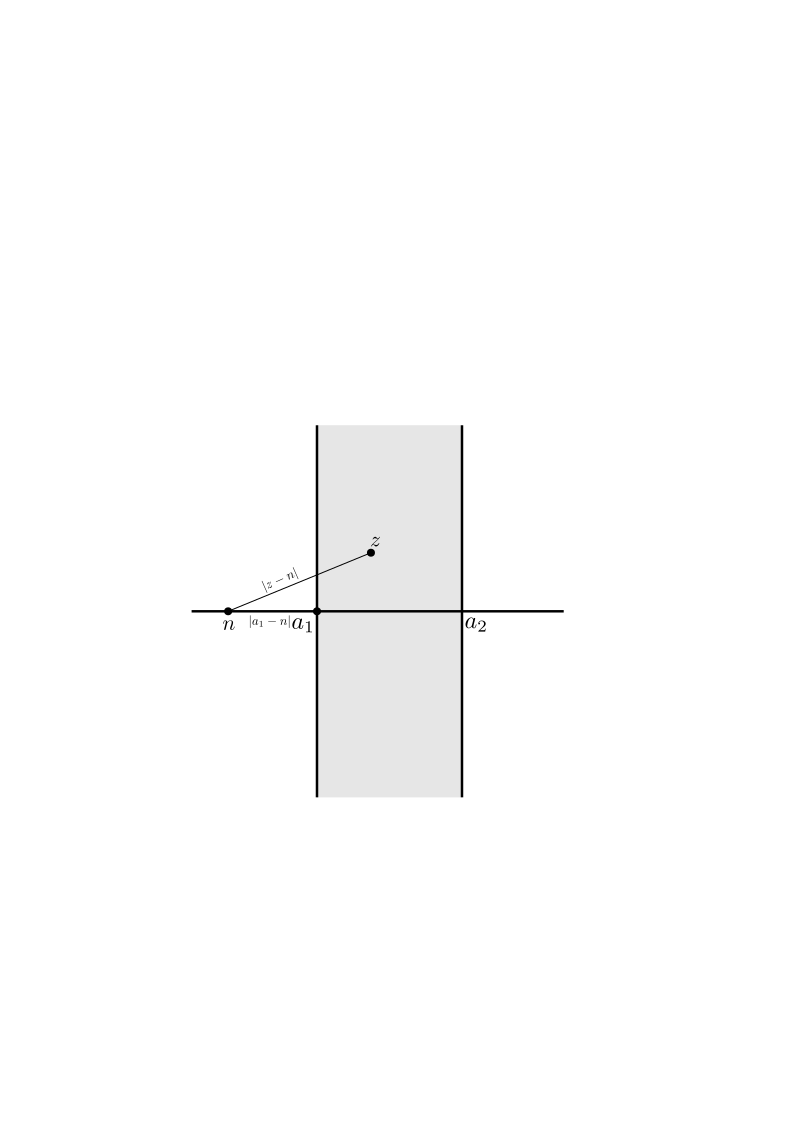
\includegraphics[scale=0.65]{Images/vertical_strip_cvgnc.png}
    \caption{The series for $f(z)$ converges on every vertical strip in the complex plane}
    \label{fig:vertical-strip-cvgnc}
\end{figure}

% TODO: Add diagram

For $n < a_1$ and $n > a_2$, the functions $1/(z - n)^2$ are holomorphic on this strip, thus we can ignore all $n$ that lie in $(a_1, a_2)$. Moreover for $n < a_1$ we have $1/\abs{z - n} < 1/\abs{a_1 - n}$ for $z$ in the strip (see \autoref{fig:vertical-strip-compare}). Therefore 
$$ \sum_{n = -\infty}^{a_1} \abs{f_n(z)} < \sum_{n = -\infty}^{a_1} \frac{1}{(a_1 - n)^2} $$
which converges as it is comparable to $\sum 1/n^2$. The analogous argument holds for $n > a_2$. Therefore the series converges to a meromorphic function.

\begin{figure}[ht]
    \centering
    \includegraphics[scale=0.75]{Images/vertical_strip_compare.png}
    \caption{We have $1/\abs{z - n} < 1/\abs{a_1 - n}$ for $n < a_1$}
    \label{fig:vertical-strip-compare}
\end{figure}

We want to find $f$ more explicitly. Let us consider what properties $f(z)$ has. We know $f$ is periodic with period 1 and it has double poles at the integers. There is another function that has these properties, namely
$$g(z) := \left( \frac{\pi}{\sin \pi z} \right)^2$$
We claim that these two functions are in fact equal.